\documentclass[a4paper,12pt,twoside]{scrreprt}
% Autor der Vorlage: Klaus Rheinberger, FH Vorarlberg
% 2017-02-20

%% Hilfe: z.B.
% empfohlener Einstieg: http://latex.tugraz.at/  
% https://de.wikibooks.org/wiki/LaTeX-Kompendium:_Schnellkurs:_Erste_Schritte
% https://de.wikibooks.org/wiki/LaTeX-Kompendium:_Schnellkurs
% https://de.wikibooks.org/wiki/LaTeX-Kompendium

%% Pakete:
% Der Befehl \usepackage[latin9]{inputenc} ermöglicht die direkte Angabe von Umlauten. Übrigens lässt sich so auch das Euro-Zeichen direkt eingeben. Auf Betriebssystemen, wie zum Beispiel allen neueren Linux-Distributionen, verwendet man statt \usepackage[latin9]{inputenc} besser \usepackage[utf8]{inputenc}, auf Applesystemen verwendet man \usepackage[macce]{inputenc} (oder das für ältere Modelle gültige \usepackage[applemac]{inputenc}).
\usepackage[utf8]{inputenc}
\usepackage[T1]{fontenc}    % Silbentrennung bei Sonderzeichen
\usepackage{graphicx}       % Bilder einbinden
\usepackage[ngerman]{babel} % Deutsche Sprachanpassungen
\usepackage{csquotes}       % When using babel or polyglossia with biblatex, loading csquotes is recommended to ensure that quoted texts are typeset according to the rules of your main language.
\usepackage{acronym}  % für optionales Abkürzungsverzeichnis
\usepackage{eurosym}  % z. B. \EUR{12345,68}
\usepackage[linktocpage=true]{hyperref} % Links z. B. \href{https://www.wikibooks.org}{Wikibooks home}
\usepackage{caption} % Abbildungslegenden
\captionsetup{format=hang, justification=raggedright}
\usepackage[style=alphabetic,citestyle=alphabetic,backend=biber]{biblatex}   % Literaturverweise
% biblatex comes with a variety of built-in bibliography/citation style families (numeric, alphabetic, authoryear, authortitle, verbose), and there's a growing number of custom styles:
% https://de.sharelatex.com/learn/Biblatex_citation_styles
% https://de.sharelatex.com/learn/Biblatex_bibliography_styles
\addbibresource{bibliography.bib}    % Zotero-Beispiele.bib ist die verwendete Bibtex-Datei 
% Anstatt die Bibtex-Datei selber zu erstellen, kann sie z. B. aus einer Zotero-Sammlung zu BibTeX exportiert werden.


%% Einstellungen:
\setcounter{secnumdepth}{4}
\setcounter{tocdepth}{4}   % Tiefe der Gliederung im In haltsverzeichnis


%% ERSETZEN VON ECKIGEN KLAMMERN:
% Ersetzen Sie den Text in den eckigen Klammern!

\begin{document}

% evtl. Sperrvermerkseite
\thispagestyle{empty}
[Achtung: Verwenden Sie einen Sperrvermerk nur in sehr gut begründeten Fällen!] 

\section*{[evtl. Sperrvermerk]}   % evtl. ersetzen durch \section*{Sperrvermerk}
Auf Wunsch der Firma [FIRMA] ist die vorliegende Arbeit bis zum [DATUM] für die öffentliche Nutzung zu sperren. 

Veröffentlichung, Vervielfältigung und Einsichtnahme sind ohne ausdrückliche Genehmigung der oben genannten Firma und der/dem Verfasser/in nicht gestattet. Der Titel der Arbeit sowie das Kurzreferat/Abstract dürfen jedoch veröffentlicht werden.

\vspace{3cm}

\noindent Dornbirn, \hfill Unterschrift der Verfasserin/des Verfassers

\vspace{2cm}

\hfill Firmenstempel\hspace{2cm}


% Titelblatt:
% \newpage\mbox{}\newpage

% force output to a right page
\cleardoublepage
\thispagestyle{empty}
\begin{titlepage}
  \begin{flushright}
  
\includegraphics[width=0.4\linewidth]{Logo-A3}
  \end{flushright}
  \begin{flushleft}
  \section*{[Titel der Arbeit]}
  \subsection*{[Untertitel der Arbeit]}
  \vspace{1cm}
  
  Masterarbeit\\
  zur Erlangung des akademischen Grades
  \vspace{0.5cm}
  
  \textbf{[z. B. Master of Science in Engineering (MSc)]}

  \vspace{1cm}
  Fachhochschule Vorarlberg\newline
  [z. B. Energietechnik und Energiewirtschaft]

  \vspace{0.5cm}
  
  Betreut von\newline
  [Name(n) der betreuenden Lehrperson(en)]
  
  \vspace{0.5cm}
  
  Vorgelegt von\newline
  [Name(n) der Verfasser/innen]\newline
  Dornbirn, [Monat Jahr]
  \end{flushleft}
\end{titlepage}


% evtl. Widmung:
\newpage
\section*{[evtl. Widmung]}   % evtl. ersetzen durch \section*{Widmung}

[Text der Widmung]

% Kurzreferat:
\newpage
\section*{Kurzreferat}

\subsection*{[Deutscher Titel Ihrer Arbeit]}

[Text des Kurzreferats]


% Abstract:
\newpage
\section*{Abstract}
\subsection*{[English Title of your thesis]}

[text of the abstract]


% evtl. Vorwort:
\newpage
\section*{[evtl. Vorwort]}   % evtl. ersetzen durch \section*{Widmung}

[Text des Vorworts]


% Inhaltsverzeichnis:
\cleardoublepage   % force output to a right page
\tableofcontents

\clearpage
\phantomsection
\addcontentsline{toc}{chapter}{Abbildungsverzeichnis}
\listoffigures

\clearpage
\phantomsection
\addcontentsline{toc}{chapter}{Tabellenverzeichnis}
\listoftables

% evtl. Abkürzungsverzeichnis:
\clearpage
\phantomsection
\addcontentsline{toc}{chapter}{[evtl. Abkürzungsverzeichnis]}  % evtl. ersetzen durch \addcontentsline{toc}{chapter}{Abkürzungsverzeichnis}
\chapter*{[evtl. Abkürzungsverzeichnis]} % evtl. ersetzen durch \chapter*{Abkürzungsverzeichnis}
\begin{acronym}[SQL]
 \acro{ETW}{Energietechnik und Energiewirtschaft}
 \acro{SQL}{Structured Query Language}
 \acro{Bash}{Bourne-again shell}
\end{acronym}

%% Die Kapitelstruktur ist mit der betreuungsperson abzustimmen!

\chapter{[Kapitel]}
Formatvorlage für den Fließtext. Formatvorlage für den Fließtext. Formatvorlage für den Fließtext. Formatvorlage für den Fließtext. Formatvorlage für den Fließtext. Formatvorlage für den Fließtext. Formatvorlage für den Fließtext. Formatvorlage für den Fließtext. Formatvorlage für den Fließtext. Formatvorlage für den Fließtext. Formatvorlage für den Fließtext.
\begin{quote}
  Formatvorlage für ein längeres direktes Zitat. Formatvorlage für ein längeres direktes Zitat. Formatvorlage für ein längeres direktes Zitat. Formatvorlage für ein längeres direktes Zitat. Formatvorlage für ein längeres direktes Zitat. Formatvorlage für ein längeres direktes Zitat….
\end{quote}

Formatvorlage für den Fließtext.
Hier eine Liste.
\begin{enumerate}
 \item Verstehen
 \item Üben
 \item Können
\end{enumerate}


\section{[Unterkapitel zweite Ebene]}
Formatvorlage für den Fließtext. Die Abbildung~\ref{fig:ex} auf Seite~\pageref{fig:ex} zeigt drei Entladungskurven eines biphasischen Defibrillators.
\begin{figure}[htb]
  \centering
  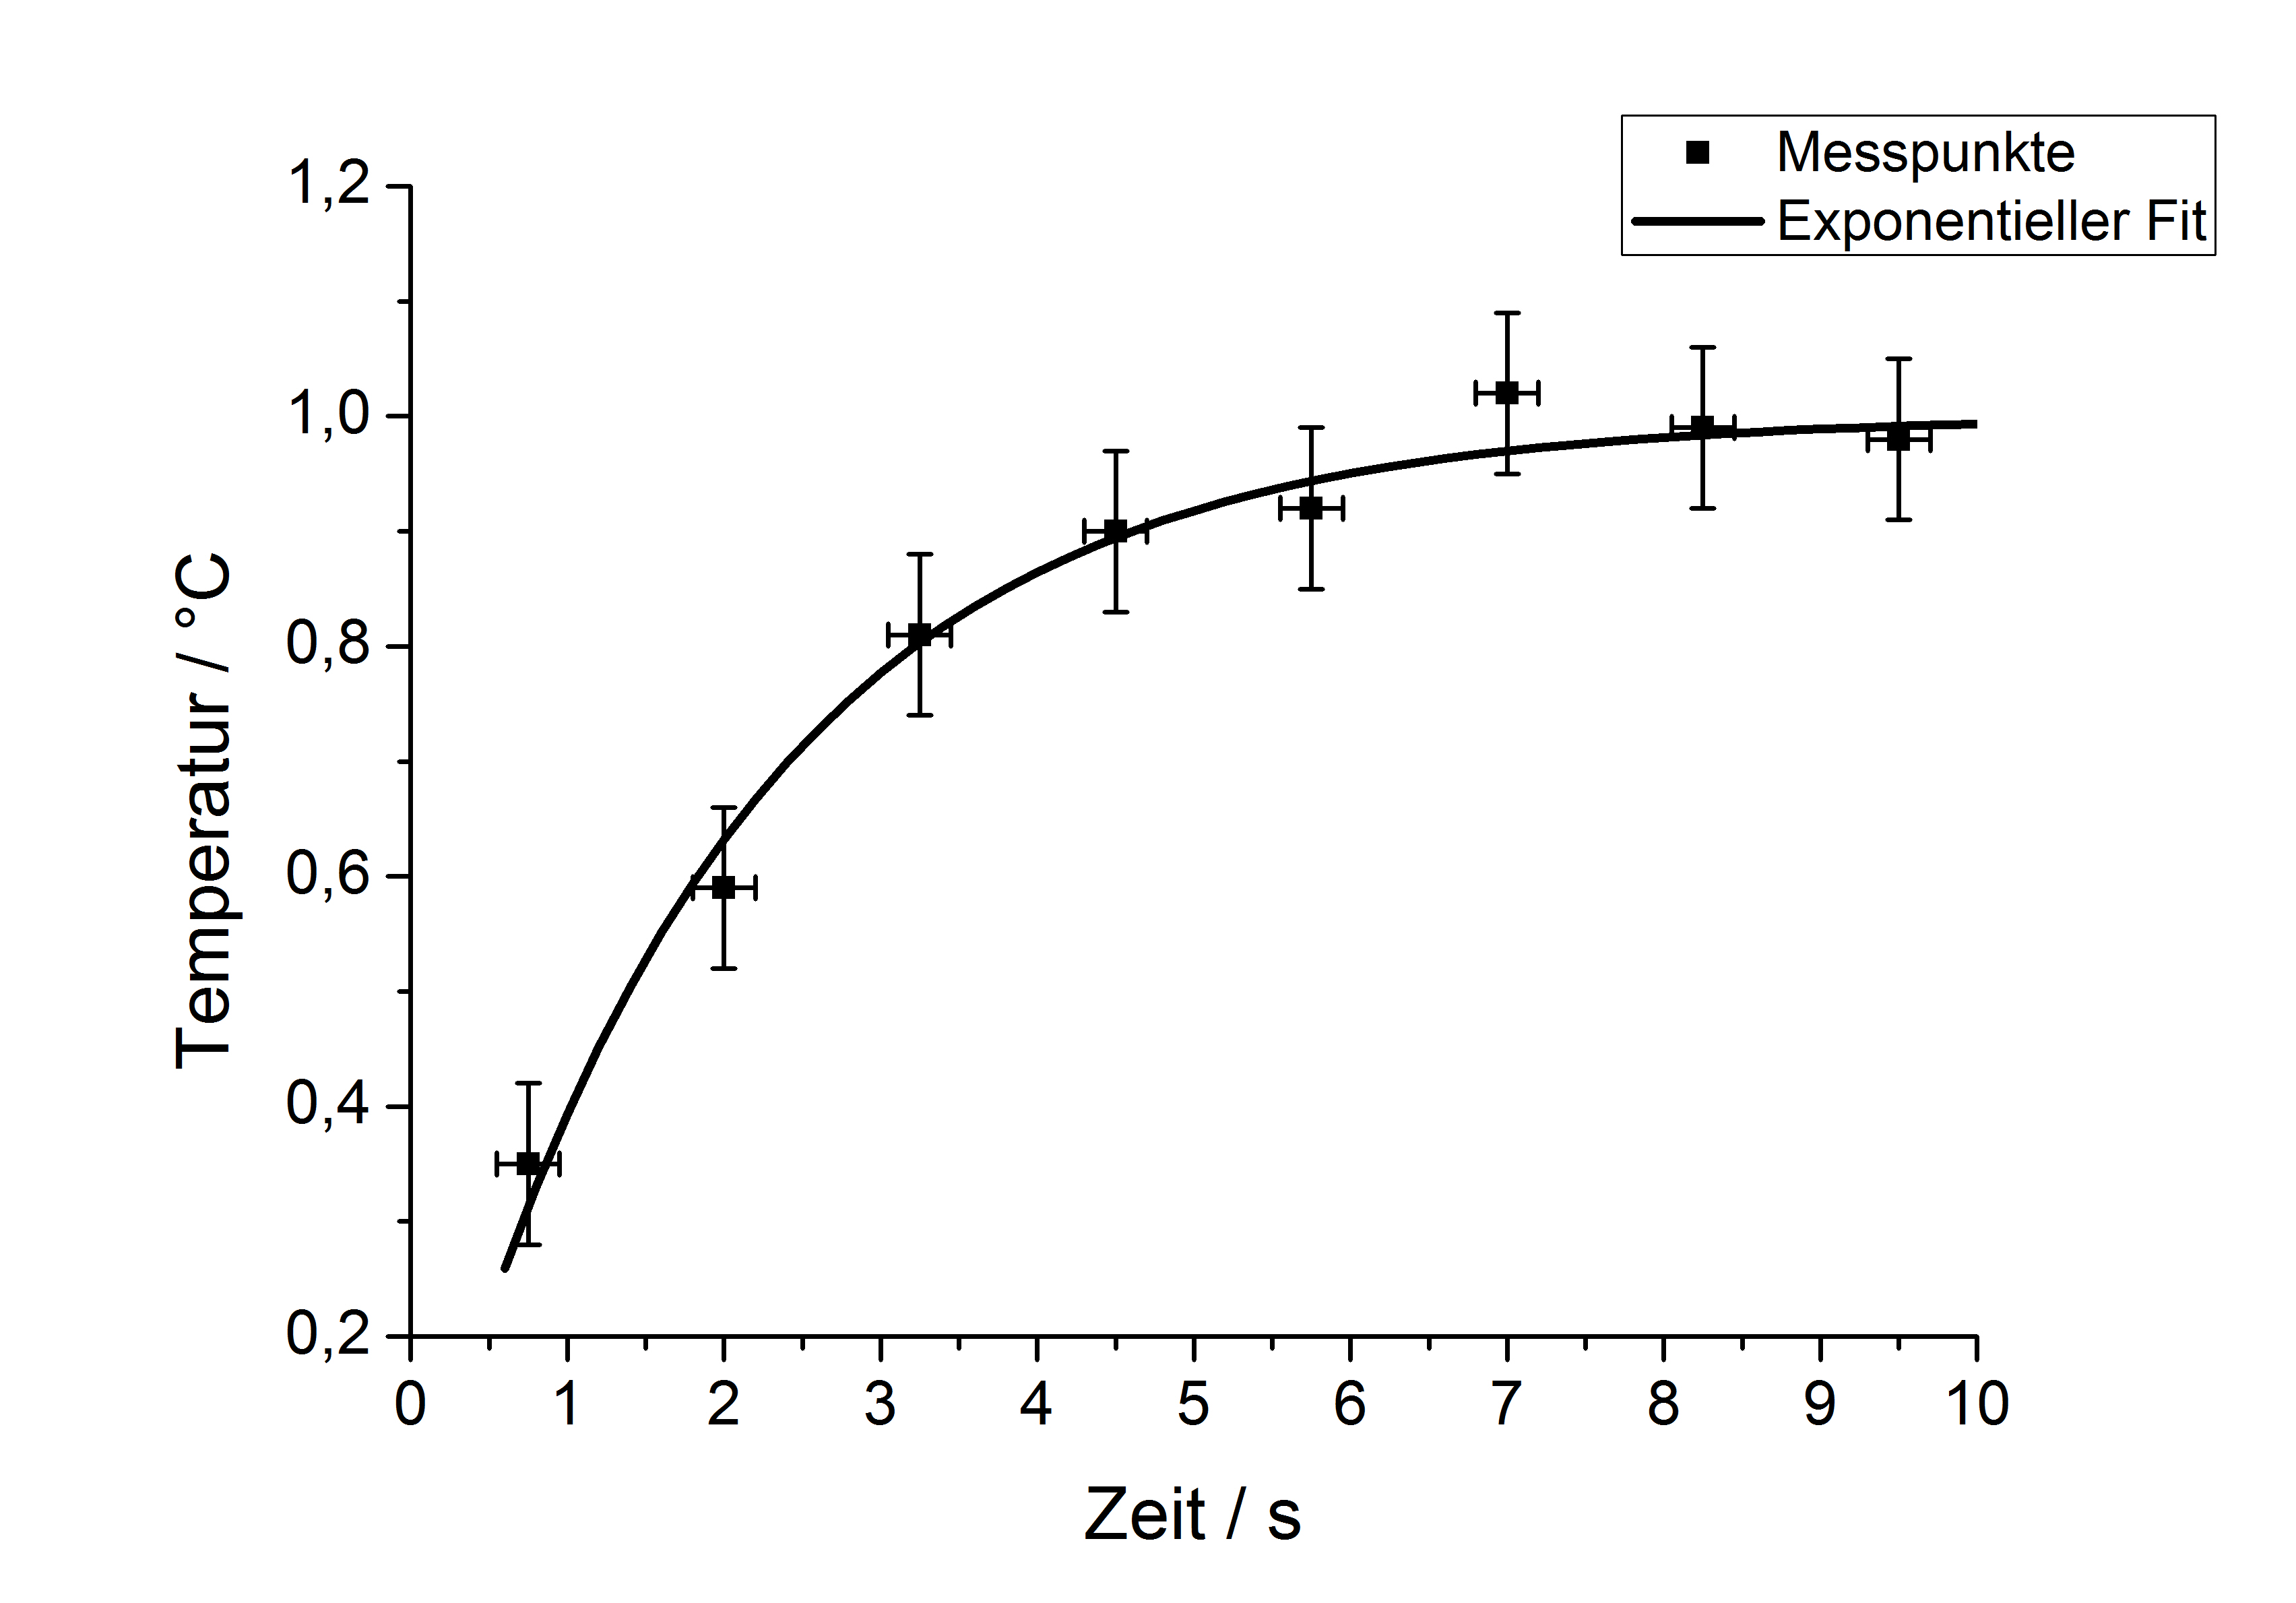
\includegraphics[width=10cm]{Amann_TechnAbb}
  \caption[Aufheizverhalten von PTFE]{Das Bild zeigt das Aufheizverhalten von PTFE\@. \\Quelle: eigene Ausarbeitung}
\label{fig:ex}
\end{figure}


\section{[Unterkapitel zweite Ebene]}
Formatvorlage für den Fließtext.
Jetzt eine Fußnote\footnote{Dies ist eine Fußnote.}
Die quadratischen Gleichung (\ref{equ:foo}) hat wieviele Nullstellen?
\begin{equation}
 \label{equ:foo}
 x^2-2x+5=0.
\end{equation}
Zwei von Einsteins berühmtesten Formeln lauten:
\begin{eqnarray*}
  E &= mc^2                                  \\
  m &= \frac{m_0}{\sqrt{1-\frac{v^2}{c^2}}}
\end{eqnarray*}


\subsection{[Unterkapitel dritte Ebene]}
Formatvorlage für den Fließtext. Hier die einfache Tabelle~\ref{tab:sp}

\begin{table}[htb]
  \centering
  \begin{tabular}{ | l | l |c|}
    \hline
    Datum      & Thema           & Raum \\
    \hline\hline
    Montag     & Graphentheorie  & U1   \\
    \hline
    Donnerstag & Algebra         & MZB23\\
    \hline
  \end{tabular}
  \caption[Stundenplan]{Stundenplan des Jahres 2030.\\Quelle: eigene Ausarbeitung}
\label{tab:sp}
\end{table}

\subsubsection{[Unterkapitel vierte Ebene]}
Formatvorlage für den Fließtext.



\section{[Unterkapitel zweite Ebene]}

Verweise: zu einem Buch mit Details~\cite[vgl.][Kapitel 2]{bathe_finite-elemente-methoden_1990} oder ohne Details~\cite{bathe_finite-elemente-methoden_1990}, ein Buchteil~\cite{areger_problem-based_2007}, eine Dissertation~\cite{sporn_interaktives_2000}, ein Dokument~\cite{industriellenvereinigung_beste_2014}, ein Enzyklopädieartikel~\cite{brockhaus_kreativitat_1872}, ein Film~\cite{de_wilde_through_2008}, ein Konferenz-Paper~\cite{weber_podcasts._2006}, ein Magazin-Artikel~\cite{autornachname1_magazinartikeltitel_1995}, ein Pordcast~\cite{paulus_horen_????}, eine Tonaufnahme~\cite{horowitz_horowitz_2003}, eine Videoaufnahme~\cite{fhvlearningsupport_was_2008}, ein Vortrag~\cite{kohls_literaturverwaltung_2008}, eine Website~\cite{wedekind_von_2008}, ein Zeitschriftenartikel~\cite{hofer_wir_2008} und ein Zeitungsartikel~\cite{schenkel_tsunami_2012}.


\chapter{[Kapitel]}

\section{[Unterkapitel zweite Ebene]}
Formatvorlage für den Fließtext.

\subsection{[Unterkapitel dritte Ebene]}
Formatvorlage für den Fließtext.

\subsubsection{[Unterkapitel vierte Ebene]}
Formatvorlage für den Fließtext.

\chapter{Einleitung}

\section[Software-Qualität]{Software-Qualität~\footcite[vgl.][Kapitel 1.2]{hoffmann_software-qualitat_2013}}

Eine mögliche Definition von Software-Qualität findet sich in der DIN-ISO-Norm 9126:

\begin{quote}
  Software-Qualität ist die Gesamtheit der Merkmale und Merkmalswerte eines Software-Produkts, die sich auf dessen Eignung beziehen, festgelegte Erfordernisse zu erfüllen.
\end{quote}

Wie aus dieser Definition schon erkennbar ist, gibt es viele unterschiedliche Kriterien, um die Qualität von Software zu bewerten.
Einige wesentliche Merkmale, um die Qualität von Software bewerten zu können, lassen sich in kunden- und herstellerorientierte Merkmale unterteilen:

\begin{description}
  \item[Kundenorientierte Merkmale] \hfill \\ Nach außen hin sichtbare Merkmale, die sich auf den kurzfristigen Erfolg der Software auswirken, da sie die Kaufentscheidung möglicher Kunden beeinflussen.
  \begin{description}
    \item[Funktionalität (Functionality, Capability)] \hfill \\ Beschreibt die Umsetzung der funktionalen Anforderungen. Fehler sind hier häufig Implementierungsfehler (sogenannte Bugs), welche durch Qualitätssicherung bereits in der Entwicklung entdeckt oder vermieden werden können. 
    \item[Laufzeit (Performance)] \hfill \\ Beschreibt die Umsetzung der Laufzeitanforderungen. Besonderes Augenmerk muss in Echtzeitsystemen auf dieses Merkmal gelegt werden.
    \item[Zuverlässigkeit (Reliability)] \hfill \\ Eine hohe Zuverlässigkeit ist in kritischen Bereichen, wie z.B. Medizintechnik oder Luftfahrt, unabdingbar. Erreicht werden kann diese aber nur durch die Optimierung einer Reihe anderer Kriterien.
    \item[Benutzbarkeit (Usability)] \hfill \\ Betrifft alle Eigenschaften eines Systems, die mit der Benutzer-Interkation in Berührung kommen.
  \end{description}
  \item[Herstellerorientierte Merkmale] \hfill \\ Sinf die inneren Merkmale, die sich auf den langfristigen Erfolg der Software auswirken und somit als Investition in die Zukunft gesehen werden sollten.
  \begin{description}
    \item[Wartbarkeit (Maintainability)] \hfill \\ Die Fähigkeit auch nach der Inbetriebnahme noch Änderungen an der Software vorzunehmen. Wird oft vernachlässigt, ist aber essentiell für langlebige Software und ein großer Vorteil gegenüber der Konkurrenz.
    \item[Transparenz (Transparency)] \hfill \\ Beschreibt, wie die nach außen hin sichtbare Funktionalität intern umgesetzt wurde. Gerade bei alternder Software, kann es zu einer Unordung kommen, welche auch Software-Entropie (Grad der Unordnung) genannt wird.
    \item[Übertragbarkeit] \hfill \\ Wird auch Portierbarkeit genannt und beschreibt die Eigenschaft einer Software, in andere Umgeungen übertragen werden zu können (z.B. 32-Bit zu 64-Bit oder Desktop zu Mobile).
    \item[Testbarkeit (Testability)] \hfill \\ Testen stellt eine große Herausforderung dar, da oft auf interne Zustände zugegriffen werden muss oder die Komplexität die möglichen Eingangskombinationen vervielfacht. Aber gerade durch Tests können Fehler frühzeitig entdeckt und behoben werden.
  \end{description}
\end{description}

Je nach Anwendungsgebiet und den Anforderungen der Software haben die Merkmale unterschiedliche Relevanz und einige können sich auch gegenseitig beeinflussen, wie aus der Korrelationsmatrix ersichtlich.

\begin{savenotes}
  \begin{figure}[H] 
    \centering
       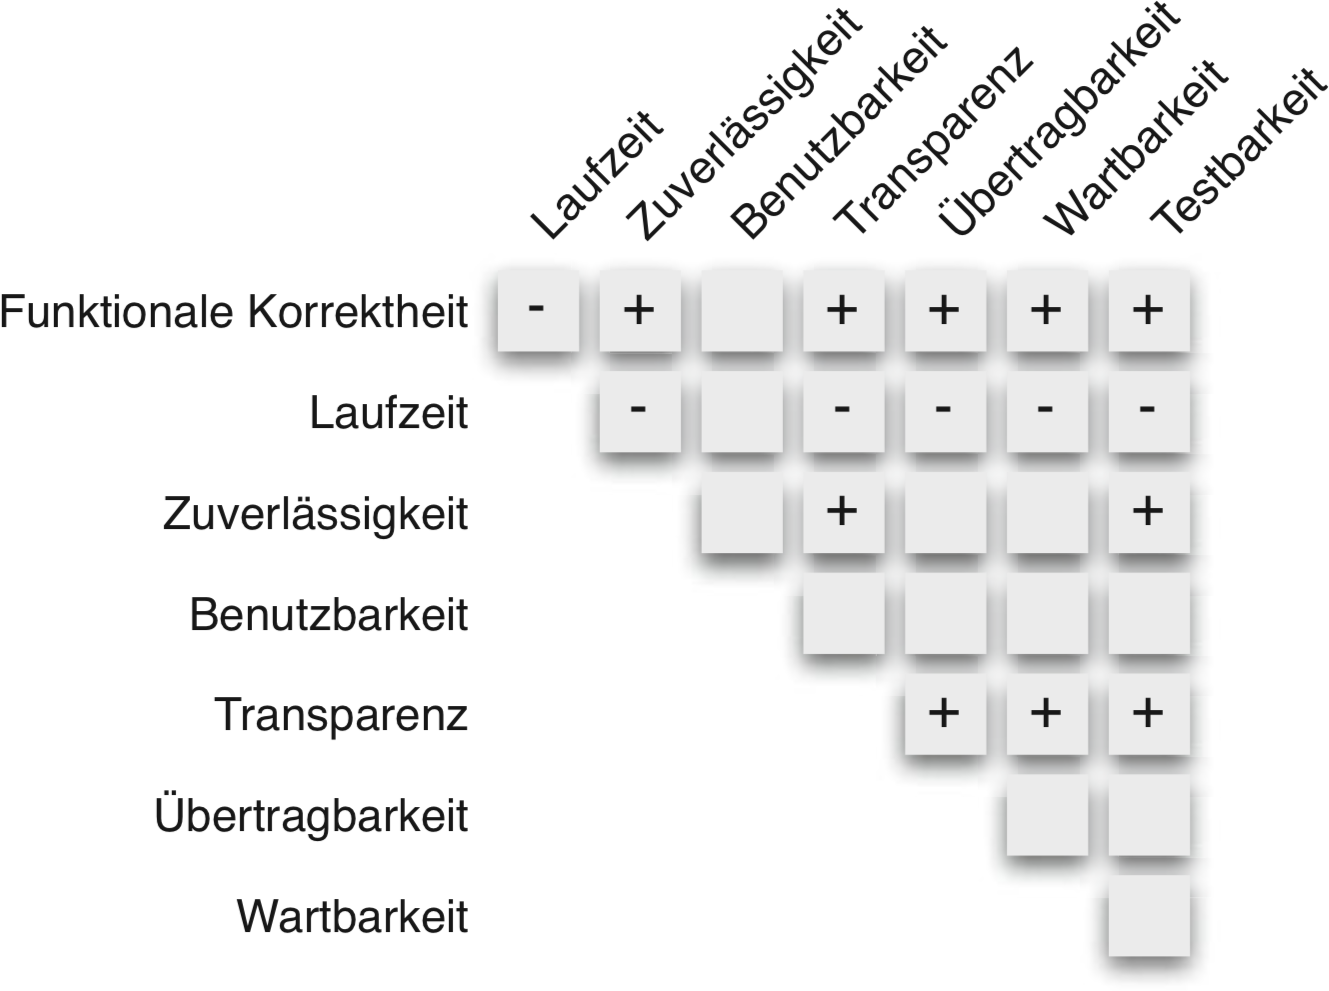
\includegraphics[width=0.6\textwidth]{img/korrelationsmatrix-kriterien.png}
    \caption[Korrelationsmatrix Qualitätskriterien]{Korrelationsmatrix Qualitätskriterien~\footcite[][S. 11, Abb. 1.3]{hoffmann_software-qualitat_2013}}
    \label{fig:JSEP Architektur}
  \end{figure}
\end{savenotes}


% Literaturverzeichnis:
\clearpage
\phantomsection
\addcontentsline{toc}{chapter}{Literaturverzeichnis}
\printbibliography


\chapter*{[evtl. Anhang]}  % evtl. ersetzen mit \chapter*{Anhang}
\addcontentsline{toc}{chapter}{[evtl. Anhang]}   % evtl. ersetzen mit \addcontentsline{toc}{chapter}{Anhang}
Formatvorlage für den Fließtext.


\chapter*{Eidesstattliche Erklärung}
\addcontentsline{toc}{chapter}{Eidesstattliche Erklärung}
Ich erkläre hiermit an Eides statt, dass ich die vorliegende Masterarbeit selbstständig und ohne Benutzung anderer als der angegebenen Hilfsmittel angefertigt habe. Die aus fremden Quellen direkt oder indirekt übernommenen Stellen sind als solche kenntlich gemacht. Die Arbeit wurde bisher weder in gleicher noch in ähnlicher Form einer anderen Prüfungsbehörde vorgelegt und auch noch nicht veröffentlicht.

\vspace{3cm}
\noindent
Dornbirn, am [Tag. Monat Jahr anführen]\hfill [Vor- und Nachname Verfasser/in]


\end{document}
